% !TEX root = machine_learning.tex
%\preface
%The backbone of these lecture notes derives from the text-book {\em The
%elements of statistical learning} by Hastie, Tibshirani and
%Friedman \cite{htf03}. There are however several additions and
%omissions. Among the additions, several details regarding kernel
%methods \cite{ss02}, some theoretical facts on nearest neighbor
%methods \cite{dgl96}, and an short review of some recent results in the estimation
%of generalization errors \cite{dgl96, bbl02}.

%In this first version, the cited literature is minimal. This will be
%extended later, but in the meanwhile, the reader is invited to refer
%to the cited textbooks for extensive bibliographies. 

%Since this is the first version of these notes, they are likely to
%contain a large number of typos and mistakes. If you spot some, I would
%be delighted to hear from you by email (laurent.younes@jhu.edu).

\chapter[Introduction: Bias and Variance]{Introduction: Bias, Variance and Density Estimation}
\label{chap:intro}



In this chapter, we illustrate the bias variance dilemma in the context of density estimation, in which problems are similar to those  encountered in classical parametric or non-parametric statistics \citep{rao1983nonparametric,dgl96,pons2011functional}. 

For density estimation, one assumes that a random variable $X$ is given with unknown p.d.f. $f$ and we want to build an estimator, i.e., a mapping $(x, T) \mapsto \hat f(x;T)$ that provides an estimation of $f(x)$ based on a training set $T = (x_1, \ldots, x_N)$ containing $N$ i.i.d. realizations of $X$ (i.e., $T$ is a realization of $\mT = (X_1, \ldots, X_N)$, $N$ independent copies of $X$). Alternatively, we will say that the mapping $T \mapsto \hf(\,\cdot\,; T)$ is an estimator of the full density $f$. Note that, to further illustrate our notation, $\hf(x;T)$ is a number while $\hf(x; \mT)$ is a random variable.



%Before starting this discussion, we introduce some notation that will be used throughout this book.
% one generally considers three main supervised estimation problems, namely:
%\begin{itemize}[leftmargin=.5cm]
%\item Density estimation: From a training set  $(x_1, \ldots, x_N)$, considered as an i.i.d. sample of a r.v. $X$, find a function $\hat f_X$ that estimate the p.d.f. of $X$. \footnote{i.i.d.: independent, identically distributed; i.i.d. sample: a realization of $N$ i.i.d. random variables; p.d.f.: probability density function; r.v.: random variable.}
%\item Regression: given a training set $(x_1, y_1), \ldots, (x_N,
%y_N)$, considered as a sample of a pair of random variables $(X,Y)$ with $x_k\in \CR$ (typically $\mR^d$) and $y_k\in \mR^q$, find a function
%$\hf_n:\mR^d \to \mR^q$ that approximates the conditional expectation $E(Y|X)$.
%\item Classification: given a training set $(x_1, y_1), \ldots, (x_N,
%y_N)$, considered as a sample of a pair of random variables $(X,Y)$
%with $x_k\in\CR$ and $y_k$ in a finite set $\CG$ of classes, find a function
%$\hf_n:\mR^d \to \CG$ which approximate the best prediction of the true class knowing $X$.
%\end{itemize}
% A large part of these notes address the the last two issues. We will also discuss unsupervised ``dimension reduction'' and clustering methods. Density estimation will, however, not be a major focus for us, except in this chapter, in which we will use it as an example to introduce the ``bias vs. variance dilemma.'' 



\section{Parameter estimation and sieves}
\label{sec:sieves} 
Parameter estimation is the most common density estimation method, in which one restrict $\hat f$ to belong to
a finite-dimensional parametric class, denoted $(f_\th, \th\in\Th)$, with $\Th\sub
\mR^p$. For example, $f_\th$ can be a family of Gaussian distributions
on $\mR^d$. With our notation, a parametric model provides estimators taking the form
\[
\hf(x; T) = f_{\hat\th(T)}(x)
\]
and the problem becomes the estimation of the parameter $\hat\th$.


There are several, well-known methods for parameter
estimation, and, since this is not the focus of the book, we only
consider the most common one, maximum likelihood, which consists in
computing $\hth$ that maximizes the log-likelihood
\begin{equation}
\label{eq:log.lik}
C(\th) = \frac{1}{N}\sum_{k=1}^N \log f_\th(x_k)\,.
\end{equation}
The resulting $\hth$ (when it exists) is called the maximum likelihood estimator of $\th$, or m.l.e.


If the true $f $ belongs to the parametric class, so that $f= f_{\th_*}$ for some $\theta_*\in \Th$, standard results in mathematical statistics \cite{bickel2015mathematical,lehmann2006theory} provide sufficient conditions for  $\hth$ to converge to $\th_*$ when $N$ tends to infinity.
However, the fact that the true p.d.f. belongs to the finite
dimensional class $(f_\th)$ is an optimistic assumption that is generally false. In this regard, the standard theorems in parametric statistics may be regarded as analyzing  a ``best case scenario,'' or as performing a ``sanity check,'' in which one asks whether, in the ideal situation in which $f$ actually belongs to the parametric class, the designed estimator has a proper behavior. In non-parametric statistics, a  parametric model can still be a plausible approach in order to approximate the true $f$, but the relevant question should then be whether $\hat f$ provides (asymptotically), the best approximation to $f$ among all  $f_\th$, $\th\in \Th$. The maximum likelihood estimator can be
analyzed from this viewpoint, if one measures the difference between two
density functions by the Kullback-Liebler divergence (also called differential entropy):
\begin{equation}
\label{eq:kl.pdf}
\KL(f \| f_\th) = \int_{\mR^d} \log \frac{f(x)}{f_\th(x)} f(x) dx
\end{equation}
which is positive unless $f=f_\th$ (and may be equal to $+\infty$). 

This expression of the divergence is a simplification of its general mea\-sure-theo\-retic definition, that we now provide for completeness---and future use. Let $\mu$ and $\nu$ be two probability measures on a set $\widetilde \Om$. One says that $\mu$ is absolutely continuous with respect to $\nu$, with notation $\mu\ll\nu$, if, for every (measurable) subset  $A \sub \widetilde \Omega$, $\nu(A) = 0$ implies $\mu(A) = 0$. The Radon-Nikodym theorem \citep{billingsley2008probability} states that $\mu\ll \nu$ is and only if there exists a non-negative function $g$ defined on $\widetilde \Omega$ such that 
\[
\mu(A) = \int_{A} g(x) d\nu(x).
\]
In terms of random variables, this says that, if $X: \Omega \to \widetilde \Omega$ and $Y: \Omega \to \widetilde \Omega$ are two random variables with respective distributions $\mu$ and $\nu$, and $\phi: \widetilde \Omega \to \mR$ is measurable, then $E(\phi(X)) = E(g(Y)\phi(Y))$. The function $g$ is called the Radon-Nikodym derivative of $\mu$ with respect to $\nu$ and is denoted $d\mu/d\nu$ (it is defined up to a modification on a set of $\nu$-probability zero). The general definition of the Kullback-Liebler divergence between $\mu$ and $\nu$ is then:
\begin{equation}
\label{eq:kl.definition}
\KL(\mu \| \nu) = \left\{
\begin{aligned}
&\int_{\tilde\Om} \left(\log \frac{d\mu}{d\nu}\right)  \frac{d\mu}{d\nu} d\nu && \text{ if } \mu \ll \nu\\
&+\infty && \text{ otherwise}
\end{aligned}
\right.
\end{equation}
In the case when $\mu = f \,dx$ and $\nu = \tilde f \,dx$ are both probability measures on $\mR^d$ with respective p.d.f.'s $f$ and $\tilde f$, $\mu \ll \nu$ means that $f/\tilde f$ is well defined everywhere except on a set of $\nu$-probability zero. It is then equal to $d\mu/d\nu$.  If $\mu\ll\nu$, we can therefore write
\[
\KL(\mu\|\nu) = \int_{\mR^d} \frac{f(x)}{\tilde f(x)} \log \bigg(\frac{f(x)}{\tf(x)}\bigg) \tilde f(x) dx = \int_{\mR^d}  \log \bigg(\frac{f(x)}{\tf(x)}\bigg) f(x) dx
\] 
and
we will make the abuse of notation of writing $\KL(f \| \tf)$ for $\KL(f\, dx\| \tf\,dx)$, which gives the expression provided in \cref{eq:kl.pdf}. 

The general definition also gives a simple expression when $\widetilde \Om$ is a finite set, with
\[
\KL(\mu\|\nu) = \sum_{x\in\widetilde\Om} \log \frac{\mu(x)}{\nu(x)} \mu(x),
\]
that we will use later in these notes (if there exists $x$ such that $\mu(x) > 0$ and $\nu(x) =0$, then $\KL(\mu\|\nu)=\infty$).  The most important property for us is that the Kullback-Liebler divergence can be used as a measure of discrepancy between two probability distribution, based on the following proposition.
\begin{proposition}
\label{prop:kl}
Let $\mu$ and $\nu$ be two probability measures on $\widetilde \Om$. Then
  $\KL(\mu\|\nu)\geq 0$ and vanishes if and only if $\mu=\nu$.
  \end{proposition}
\begin{proof}
Assume that $\mu\ll\nu$ since the statement is obvious otherwise and let $g = d\mu/d\nu$. We have $\int_{\widetilde \Om} g d\nu = 1$ (since, by definition, it is equal to $\mu(\widetilde \Omega)$) so that 
\[
\KL(\mu\|\nu) = \int_{\widetilde \Omega} (g\log g + 1 - g) d\nu.
\] 
We have $t\log t + 1-t \geq 0$ with equality if and only $t=1$ (the proof being left to the reader) so that $\KL(\mu\|\nu) = 0$ if and only if $g=1$ with $\nu$-probability one, i.e., if and only if $\mu=\nu$. 
\end{proof}
\bigskip



Minimizing $\KL(f\| f_\th)$ with respect to $\th$ is equivalent to maximizing
$$
E_f(\log f_\th) = \int_{\mR^d} \log f_\th(x) f(x) dx\,,
$$
and
an empirical evaluation of this expectation is
$\frac{1}{N} \sum_{k=1}^N \log f_\th(x_k)$, which provides the maximum
likelihood method. Seen in this context, consistency of the maximum likelihood estimator states that this estimator almost surely converges to a best approximator of
the true $f$ in the class $(f_\th, \th\in\Th)$. More precisely, if one assumes that the function $\theta \mapsto \log f_\th(x)$ is continuous\footnote{Upper-semi continuous is  sufficient.} in $\th$ for almost all $x$ and that, for all $\th \in \Th$, there exists a small enough $\de >0$ such that
\[
\int_{\mR^d} \Big(\sup_{|\th'-\th|<\de} \log f_{\th'}(x)\Big)\, f(x)\, dx  < \infty
\]
then, letting $\Th_*$ denote the set of maximizers of $E_f(\log f_\th)$, and assuming that it is not empty, the maximum likelihood estimator $\hth_N$ is such that, for all $\ep>0$ and all compact subsets $K\sub \Th$, 
\[
\lim_{N\to \infty} \myP\big(d(\hth_N, \Th_*) > \ep \text{ and } \hth_N\in K\big) \to 0
\]
where $d(\hth_N, \Th_*)$ is the Euclidean distance between $\hth_N$ and the set $\Th_*$. 
The interested reader can refer to \citet{van2000asymptotic}, Theorem 5.14, for a proof of this statement. Note that this assertion does not exclude the situation in which $\hth_N$ goes to infinity (i.e., steps out of ever compact subset $K$ in $\Th$), and the boundedness of the m.l.e. is either asserted from additional properties of the likelihood, or by simply restricting $\Th$ to be a compact set.

If $\Th_* = \{\th_*\}$ and the m.l.e. almost surely converges to $\th_*$, the speed of convergence can also be quantified by a central limit theorem (see \citet{van2000asymptotic}, Theorem 5.23) ensuring that, in standard cases $\sqrt N(\hth_N - \th_*)$ converges to a normal distribution. 

%
%
%\section{Asymptotics of Maximum Likelihood Estimation}
%Here is a simple version of the consistency theorem for the m.l.e. (see \cite{van2000asymptotic} for more general results).
%\begin{theorem}
%\label{th.max.lik.cons}
%Assume that $\Th$ is a compact subset of $\mR^p$, and that $\th \mapsto \log
%f_\th(x)$ is
%continuous in $\th$ uniformly with respect to $x$. 
%
%Let $\hth_N$ be a maximizer of the likelihood based on the observations
%$X_1, \ldots, X_N$. Then, for any $\ep >0$,
%$$
%\lim_{N\to\infty} P\left(K( f_{\hth}|f) \geq  \inf_{\th \in \Th}K(f_\th,
%f)+\ep\right) = 0
%$$
%almost surely.
%\end{theorem}
%The theorem's assumption means that, for all $\ep >0$, there exists $\de$ such that,
%for all $x\in\mR^d$:
%$$
%|\th-\th'|\leq \de \Rightarrow |\log f_\th(x) - \log f_{\th'}(x)| \leq \ep
%$$
%
%\begin{proof}
%The proof can be reduced to
%showing that, for $\ep >0$ (letting $h_\th(x) = \log f_\th(x)$)
%\begin{equation}
%\label{eq:sup.th}
%P\left(\sup_{\th\in\Th} \left|\frac{1}{N} \sum_{i=1}^N h_\th(X_i) - E_f(h_\th)\right|
%> \ep\right) \to 0
%\end{equation}
%when $N$ tends to infinity. Indeed, if this is true, then, for any
%$\th_*\in \Th$ we have, using the notation in  \eqref{eq:log.lik},
%\begin{eqnarray*}
%E_f(h_{\th_*}) - E_f(h_{\hth_N})  &=&  E_f(h_{\th_*}) - C(\th_*) + C(\th_*)
%- C(\hth_N) + C(\hth_N) -  E_f(h_{\hth_N})\\
%&\leq&  E_f(h_{\th_*}) - C(\th_*) + C(\hth_N) -  E_f(h_{\hth_N})\\
%&\leq&  2 \sup_{\th} |E_f(h_{\th}) - C(\th)|,
%\end{eqnarray*}
%which implies, maximizing the first term with respect to $\th_*$:
%$$
%\max_{\th\in\Th} E_f(h_{\th}) - E_f(h_{\hth_N})  \leq 2 \sup_{\th}
%|E_f(h_{\th}) - C(\th)|
%$$
%Therefore, if \eqref{eq:sup.th} is true, we have, for all $\ep >0$
%$$
%P\left(E(h_{\hth_N}) \leq \max_{\th} E_f(h_{\th})  - \epsilon\right) \to 0
%$$
%when $N$ tends to infinity, which proves that the maximum likelihood
%estimator is arbitrarily close to the best approximator in $\Th$ when
%$N$ tends to infinity.
%
%
%So, it remains to prove \eqref{eq:sup.th}, which states the uniform convergence (in probability) of
%the empirical estimates to their expectation. 
%Consider a finite covering of
%$\Th$ with balls of radius $\de$. Let $n_\de$ be the number of needed
%balls and $\th_1, \ldots, \th_{n_\de}$ their centers. Define, for short, $\De_\th = C(\th) -
%E(h_\th)$. We have
%\begin{eqnarray*}
%P (\sup_{\th\in \Th} |\De_\th| > \ep) &=& P( \exists i, \sup_{B(\th_i,
%\de)} |\De_\th| \geq \ep )
%\\
%&\leq & n_{\de} \sup_{i=1, \ldots,n_\de} P(\sup_{|\th'-\th_i| \leq \de} |\De_{\th'}|
%\geq \ep)
%\end{eqnarray*}
%Now, having assumed that $h_\th$ is continuous in $\th$, uniformly
%with respect to $x$, we can choose $\de$ small enough to ensure that, for
%$|\th-\th'|\leq \de$, we have
%$|\De_\th - \De_{\th'}|\leq \ep/2$. This fixes also the $\th_i$'s, and
%we have in this case
%$$
%\sup_{|\th'-\th_i| \leq \de} |\De_{\th'}|
%\geq \ep \Rightarrow \exists i, \De_{\th_i} \geq \ep/2,$$ 
%so that 
%$$
%P (\sup_{\th\in \Th} |\De_\th| > \ep)  \leq  n_{\de} \sup_{i=1,
%\ldots, n_\de} P(|\De_{\th_i}|
%\geq \ep/2).
%$$
%Letting now $N$ tend to infinity, the law of large numbers implies
%that the upper bound tends to 0.
%\end{proof}
%
%We have just obtained the fact that, under some smoothness assumption
%on the log-density, the MLE asymptotically achieves the best
%approximation error in the model $\Th$. If it is assumed that there is
%a unique best parameter $\th_*$, then $\hth_N \to \th_*$ (in
%probability) when $N\to\infty$.
%
%\bigskip
%
%Consistency of the MLE can be completed with asymptotic normality, as
%we now describe.
%We restrict to the case when there is a unique best
%approximator, $\th_*$, such that $\hth_N\to \th_*$ (almost surely),
%and that {\em $\th_*$
%is in the interior of $\Th$}. We also assume
%enough derivatives (three) in $\th$ of the log-density, and that they are
%uniformly bounded in $x, \th$. Then the following theorem holds, with
%$h_\th = \log f_\th$.
%
%\begin{theorem}
%\label{th:max.lik.norm}
%With the previous assumptions, and if the matrix $S := E_f(\prt_\th^2
%h_{\th_*})$ is invertible, the maximum likelihood estimator is
%asymptotically normal. More precisely, the random variable
%$\sqrt{N}(\hth_N - \th^*)$ converges in distribution to $\mathcal N(0,
%S^{-1}\Sig
%S^{-1})$ with
%$\Sig = E_f(\nabla_\th h_{\th_*}\nabla_\th h_{\th_*}^T).$
%\end{theorem}
%Here $\prt_\th^2 h_\th$ refers to the symmetric matrix containing all partial second derivatives of $h_\th$ with respect to $\th$, and $\nabla_\th h_\th$ is the column vector of first partial derivatives. Since derivatives are all with respect to $\th$, we will omit this subscript in the proof that follows.
%
%\begin{proof}
%Because we assume
%that $\hth_N$ is, for large enough $N$, an interior point of $\Th$, the derivative of the log-likelihood in $\th$ must
%vanish at $\hth_N$. Making a first order expansion of this derivative,
%we have
%$$
%\frac{1}{N} \sum_{i=1}^N \nabla h_{\th_*}(X_i) + \frac{1}{N}
%\sum_{i=1}^N \prt^2 h_{\th_*}(X_i) (\hth_N - \th_*) = O(|\th_* -
%\hth_N|^2)
%$$
%Multiply this by $\sqrt{N}$ to obtain
%$$
%\frac{1}{\sqrt{N}} \sum_{i=1}^N \nabla h_{\th_*}(X_i) + \frac{1}{N}
%\sum_{i=1}^N \prt^2 h_{\th_*}(X_i) (\sqrt{N}(\hth_N - \th_*)) = O(\sqrt{N}|\th_* -
%\hth_N|^2).
%$$
%By the central limit theorem, the first term (which will be denoted
%$Z_N$) converges in distribution
%to $\CN(m ,\Sig)$, with $m = E_f(\nabla h_{\th_*})$. We  have
%$m  = 0$, however, because $\th_*$ maximizes
%$E(h_\th)$ and $\th_*$ is interior to $\th$. The limit covariance,
%$\Sig$, is given by
%$$
%\Sig = E_f(\nabla h_{\th_*}\nabla h_{\th_*}^T)\,.
%$$
%
%From the law of large numbers $S_N = \frac{1}{N}
%\sum_{i=1}^N \prt^2 h_{\th_*}(X_i) \to S$ almost
%surely. So, letting $U_N = \sqrt{N}(\hth_N - \th_*)$, we have
%$$
%S_N^{-1} Z_N + U_N = |U_N| \ep_N
%$$
%with $|\ep_N| = O(|\th_*-\hth_N|) \to 0$. 
%This can be used (we skip the argument) to prove that $\ep_N|U_N|\to
%0$ and that  $U_N$ converges in distribution to $\CN(0, S^{-1}\Sig
%S^{-1})$.
%\end{proof}
%
%
%\noindent{\bf Note:} When the true $f$ is indeed equal to $f_{\th_*}$ (the usual
%assumption of parametric statistics), a standard computation proves
%that $S  = - \Sig$ which implies that the limit covariance matrix is $-S^{-1}$
%and that the MLE asymptotically achieves the Cramer-Rao lower-bound. 
%
%
%\section{Non parametric density estimation}

Even though these results relate our present subject
to classical parametric statistics, they are not sufficient for our purpose,
because, when $f\neq f_{\th_*}$, the convergence of the m.l.e. to the best
approximator in $\Th$ still leaves a gap in the estimation of $f$. This
gap is often called the {\em bias} of the class $(f_\th, \th\in \Th)$. One can reduce it
 by considering larger classes (e.g., with more dimensions), but the larger the class, the less accurate the estimation of the best approximator becomes for a fixed sample size (the estimator has a larger
{\em variance}). This issue is known as the ``bias vs.\! variance dilemma,'' and to address it, it is necessary  to adjust the
class $\Th$ to the sample size in order to optimally balance the two types of error (and all non-parametric estimation methods have at least one mechanism that allows for this). When the ``tuning parameter''  is the dimension of $\Th$, the overall approach is often referred to as the  {\em method of sieves} \cite{grenander1981abstract,geman1982nonparametric}, in which  the dimension of $\Th$ is increased as a function of $N$ in a suitable way.

Gaussian mixture models provide one of the most popular choices with the me\-thod of sieves. Modeling in this setting typically follows some variation of the following construction.
Fix a sequence $(m_N, N\geq 1)$ and let
%\footnote{In these notes, we use single bars to denote finite dimensional norm, e.g., $|x|^2 = x^Tx$. Double bars will be reserved for infinite dimensions.}
\begin{multline}
\label{eq:MoG.model}
\Th_N =  \Big\{f: f(x) =  \sum_{j=1}^{m_N} \al_j
\frac{e^{-|x-\mu_j|^2/2\sig^2}}{(2\pi\sig^2)^{d/2}},\\
 \mu_1, \ldots,
\mu_{m_N}\in\mR^d, 
\al_1 + \cdots + \al_{m_N} = 1, \al_1, \ldots, \alpha_{m_N} \in [0, +\infty), \sig>0\Big\}.
\end{multline}
There are therefore $(d+1) m_N$ free parameters in $\Th_N$. The integer $m_N$ allows one to adjust the dimension of $\Th_N$ and therefore controls the bias-variance trade-off. If  $m_N$ tends to infinity ``slowly enough,'' the m.l.e. will converges (almost surely) to the true p.d.f. $f$ \citep{geman1982nonparametric}.  However, determining optimal sequences $N \to m_N$ remains a challenging and largely unsolved  problem.

In practice the computation of  the
m.l.e. in this context uses an algorithm called {\em EM}, for expectation-maximization. This algorithm will be described later in \cref{chap:var.bayes}.

\section{Kernel density  estimation}
Kernel density estimators \cite{parzen1962estimation,sheather1991reliable,silverman1998density} provide alternatives to the method of sieves. They also lend themselves to some analytical developments that provide elementary illustrations of the bias-variance dilemma.

Define a kernel function as a function $K: \mR^d \to [0, +\infty)$ such that
\begin{equation}
\label{eq:kernel.density.def}
\int_{\mR^d} K(x) dx = 1,\quad \int_{\mR^d} |x| K(x)\, dx <\infty, \quad \int_{\mR^d} x K(x)\, dx = 0.
\end{equation}
Note that the third equation is satisfied, in particular, when $K$ is an even function, i.e., $K(-x) = K(x)$. 

Given $K$ and a scalar  $\sig >0$, the rescaled kernel is defined by
\[
K_\sig(x) = \frac{1}{\sig^d} K\left(\frac x \sig\right).
\]
Using the change of variable $y = x/\sig$ (so that $dy =
dx/\sig^d$) one sees that $K_\sig$ satisfies \cref{eq:kernel.density.def} as soon as $K$ does.

Based on a training set $T = (x_1, \ldots, x_N)$, the kernel density estimator defines the family of densities
$$
\hat f_\sig(x; T)  = \frac{1}{N} \sum_{k=1}^N K_\sig(x-x_k)
$$
One has 
\[
\int_{\mR^d} K_\sig(x-x_k)\, dx = 1
\]
so that it is clear that $\hat f_\sig$ is a p.d.f. In addition, 
\[
\int_{\mR^d} xK_\sig(x-x_k)\, dx = \int_{\mR^d} (y+x_k)K_\sig(y)\, dy = x_k
\]
so that 
\[
\int_{\mR^d} x \hf_\sig(x;T)\, dx = \bar x
\]
where $\bar x = (x_1 + \cdots + x_N)/N$.



A typical choice for $K$ is a Gaussian kernel, $K(y) =
e^{-|y|^2/2}/(2\pi)^{d/2}$. In this case, the estimated density is a sum
of bumps centered at the data points $x_1, \ldots, x_N$. The width of
the bumps is controlled by the parameter $\sig$.  A small $\sig$
implies less rigidity in the model, which will therefore be more
affected by changes in the data: the estimated density will have a
larger variance. The converse is true for large $\sig$, at the cost of
being less able to adapt to variations in the true density: the model
has a larger bias (see \cref{fig:kde.1} and \cref{fig:kde.2}).


\begin{figure}
\centering
\begin{tabular}{cc}
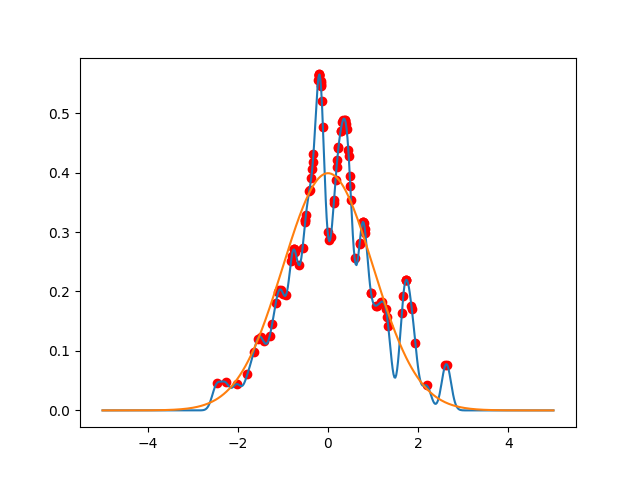
\includegraphics[trim=1cm 0cm 1cm 0cm,clip,height=0.2\textheight]{Figures/kde_gauss_0p1.png}
&
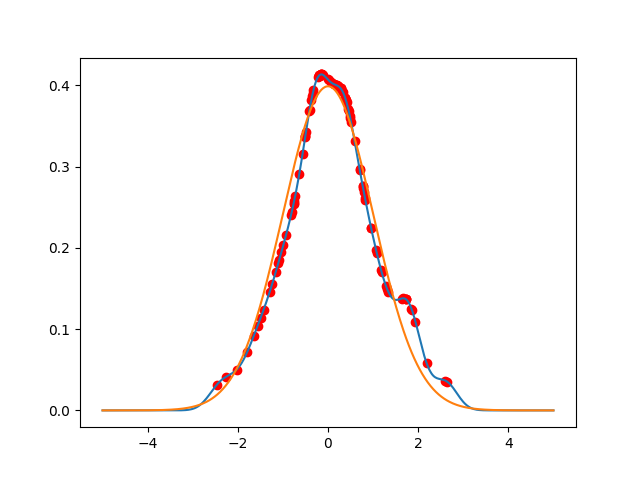
\includegraphics[trim=1cm 0cm 1cm 0cm,clip,height=0.2\textheight]{Figures/kde_gauss_0p25.png}\\
\small $\sig = 0.1$ & \small $\sig = 0.25$\\

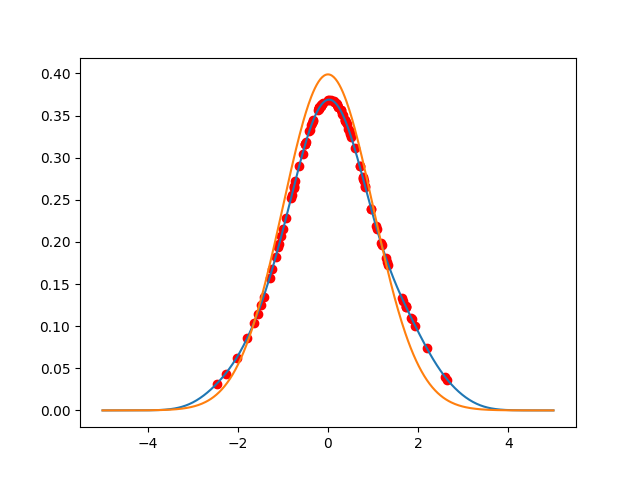
\includegraphics[trim=1cm 0cm 1cm 0cm,clip,height=0.2\textheight]{Figures/kde_gauss_0p5.png}
&
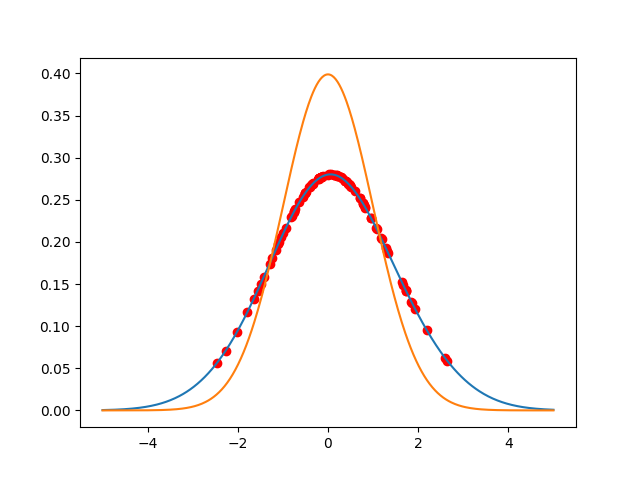
\includegraphics[trim=1cm 0cm 1cm 0cm,clip,height=0.2\textheight]{Figures/kde_gauss_1p0.png}\\
\small $\sig = 0.5$ & \small $\sig = 1.0$
\end{tabular}
\caption{\label{fig:kde.1} Kernel density estimators using a Gaussian kernel and various values of $\sig$ when the true distribution of the data is a standard Gaussian (Orange: true density; Blue: estimated density,  Red dots: training data).}
\end{figure}

\begin{figure}
\centering
\begin{tabular}{cc}
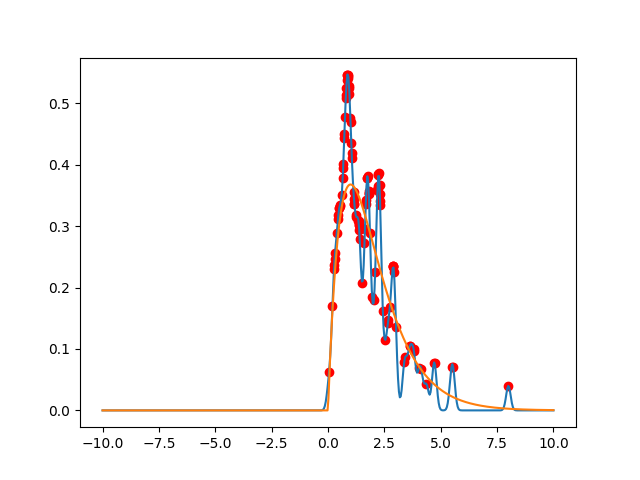
\includegraphics[trim=1cm 0cm 1cm 0cm,clip,height=0.2\textheight]{Figures/kde_gamma_0p1.png}
&
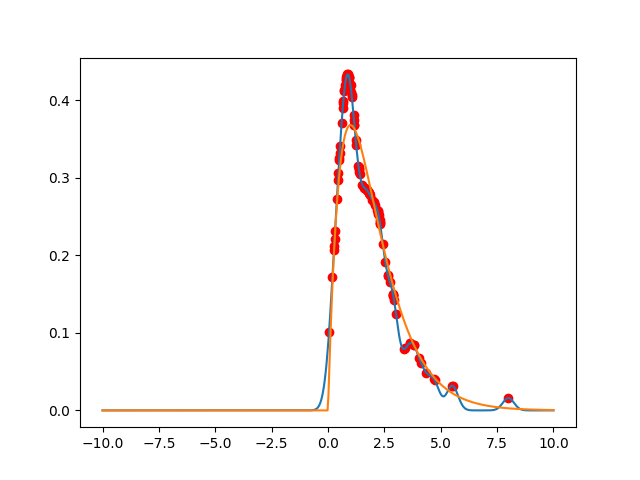
\includegraphics[trim=1cm 0cm 1cm 0cm,clip,height=0.2\textheight]{Figures/kde_gamma_0p25.png}\\
\small $\sig = 0.1$ & \small $\sig = 0.25$
\\
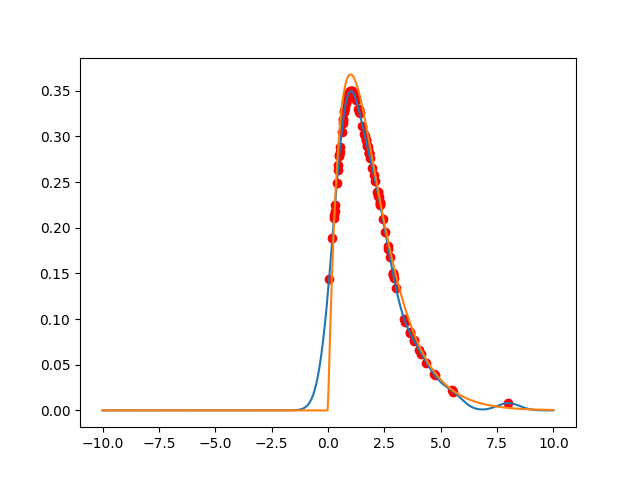
\includegraphics[trim=1cm 0cm 1cm 0cm,clip,height=0.2\textheight]{Figures/kde_gamma_0p5.png}
&
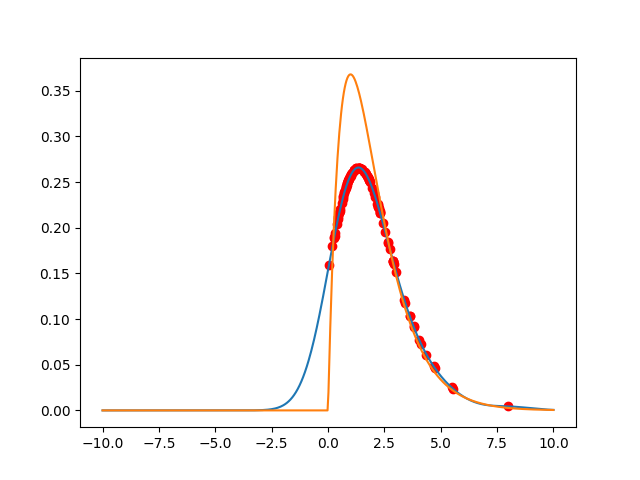
\includegraphics[trim=1cm 0cm 1cm 0cm,clip,height=0.2\textheight]{Figures/kde_gamma_1p0.png}\\
\small $\sig = 0.5$ & \small $\sig = 1.0$
\end{tabular}
\caption{\label{fig:kde.2} Kernel density estimators using a Gaussian kernel and various values of $\sig$ when the true distribution of the data is a Gamma distribution with parameter 2 (Orange: true density; Blue: estimated density, Red dots: training data).}
\end{figure}


As we now show, in order to get a consistent estimator, one needs to let  $\sig = \sig_N$ depend on the size of
the training set. 
%In particular, it can be shown that, as soon as
%$N\sig_N^d$ tends to infinity and $\sig_N$ tends to 0, the pointwise
%estimation $\hf_N(x) $ converges to $f(x)$. 
%Let us justify this with an
%informal computation. 
We have, taking expectations with respect to training data, 
\begin{eqnarray*}
E(\hf_\sig(x;\mT)) &=& \frac{1}{N\sig^d} \sum_{k=1}^N E\big
(K((x-X_k)/\sig)\big)\\
&=& \frac{1}{\sig^d} \int_{\mR^d} K((x-y)/\sig) f(y) dy\\
&=& \int_{\mR^d} K(z) f(x-\sig z) dz
\end{eqnarray*}
The bias of the estimator, i.e., the average difference between $\hf_\sig(x;\mT)$ and
$f(x)$ is therefore given by
$$
E(\hf_\sig(x;\mT)) - f(x) = \int_{\mR^d} K(z) (f(x-\sig z) - f(x)) dz.
$$
Interestingly, this bias does not depend on $N$, but only on $\sig$, and it is clear that, under mild continuity assumptions on $f$, it will go to zero with $\sig$. 

The variance of $\hf_\sig(x;\mT)$ is given by
$$
\var(\hf_\sig(x;\mT)) = \frac{1}{N\sig^{2d}} \var(K((x-X)/\sig))
$$
with
\begin{eqnarray*}
\frac{1}{N\sig^{2d}} \var(K((x-X)/\sig)) &=& \frac{1}{N\sig^{2d}} \int_\mR^d
K((x-y)/\sig)^2 f(y) dy \\
&& - \frac{1}{N\sig^{2d}} \left(\int_{\mR^d}
K((x-y)/\sig) f(y) dy\right)^2\\
&=& \frac{1}{N\sig^d} \int_{\mR^d} K(z)^2 f(x-\sig z) dz - \frac1N
\left(\int_{\mR^d}
K(z) f(x-\sig z) dz\right)^2
\end{eqnarray*}
The total mean-square error of the estimator is
$$
\myE((\hf_\sig(x) - f(x))^2) =  \var(\hf_\sig(x)) + (\myE(\hf_\sig(x)) -
f(x))^2.
$$
Clearly, this error cannot go to zero unless we allow $\sig = \sig_N$ to depend on $N$. For the bias term to go to zero, we know that we need $\sig_N \to 0$, in which case we can expect the second term in the variance to decrease like $1/N$, while, for the first term to go to zero, we need $N\sig_N^d$ to go to infinity. This illustrates the bias-variance dilemma: $\sig_N$ must go to zero in order to cancel the bias, but not too fast in order to also cancel the variance. There is, for each $N$, an optimal value of $\sig$ that minimizes the error, and we now proceed to a more detailed analysis and make this statement a little more precise.

Let us make a
Taylor expansion of both bias and variance, assuming that $f$ has at least three bounded derivatives and that $\int_{\mR^d} |x|^3 K(x) \,dx < \infty$.
We can write
$$
f(x-\sig z) = f(x) - \sig z^T \nabla f(x) + \frac{\sig^2}{2} z^T \nabla^2f(x) z +
O(\sig^3|z|^3),
$$ 
where $\nabla^2f(x)$ denotes the matrix of second derivatives of $f$ at $x$.
Since $\int zK(z) dz = 0$, this gives
$$
\myE(\hf_\sig(x;\mT)) - f(x) = \frac{\sig^2}{2} M_f (x) + o(\sig^2)
$$
with $M_f = \int K(z)\, z^T \nabla^2f(x) z\, dz$. Similarly, letting $S = \int K^2(z) \, dz$,
$$
\var(\hf_\sig(x)) = \frac{1}{N\sig^d} \big(S f(x) +  o(\sig^d + \sig^2)\big).
$$
%So the bias tends to 0 if $\sig\to 0$, and so does the variance if $N\sig^d\to\infty$. 
Assuming that $f(x)>0$, we can obtain an asymptotically optimal value for
$\sig$ by minimizing the leading terms of the mean square error, namely
$$
\frac{\sig^4}{4} M^2_f  + \frac{S}{N\sig^d} f(x)
$$
which yields $\sig_N = O(N^{-1/(d+4)})$ and 
$$
\myE((\hf_{\sig_N}(x; \mT) - f(x))^2) = O(N^{-4/(d+4)}).
$$

If $f$ has $r+1$
derivatives, and $K$ has $r-1$ vanishing moments
(this excludes the Gaussian kernel) one can reduce this error to  $N^{- \frac{2r}{2r+d}}$.  These rates can be shown to be
``optimal,'' in the ``min-max'' sense, which roughly expresses the fact that,  for any other
estimator, there exists a function $f$ for which the convergence speed
is at least as ``bad'' as the one obtained for kernel density estimation.
\bigskip

This result  says that, in order to obtain a
given accuracy $\ep$ in the worst case scenario, $N$ should be chosen of order $(1/\ep)^{1 + (d/2r)}$
which grows exponentially fast with the dimension. This is the {\em
curse of dimensionality} which essentially states that the issue of
density estimation may be intractable in large dimensions. The
same statement is true also for  most other types of machine learning problems. Since machine learning essentially deals with high-dimensional data, this issue can be problematic. 

Obviously, because the min-max theory is a worst-case analysis, not all situations will be intractable for a given estimator, and some cases that are challenging for one of them may be quite simple for others: even though all estimators are ``cursed,'' the way each of them is cursed differs. Moreover, while many estimators are optimal in the min-max sense, this theory does not give any information on ``how often''  an estimator performs better than its worst case, or how it will perform on a given class of problems. (For kernel density estimation, however, what we found was almost universal with respect to the unknown density $f$, which indicates that this estimator is not a good choice in large dimensions.)

Another important point with this curse of dimensionality is that data may very often appear to be high dimensional while it has a simple, low-dimensional structure, maybe because many dimensions are irrelevant to the problem (they contain, for example, just random noise), or because the data is supported by a non-linear low-dimensional space, such as a curve or a surface. This information is, of course, not available to the analysis, but can sometimes be inferred using some of the dimension reduction methods that will be discussed later in \cref{chap:dim.red}. Sometimes, and this is also important, information on the data structure can be provided by domain knowledge, that is, by elements, provided by experts, that specify how the data has been generated (such as underlying equations) and reasonable hypotheses that are made in the field. This source of information should never be ignored in practice.



